\section{Workflow}
As you will see better in Chapter~\ref{chapter:use_cases} dedicated to practical use cases, my internship has focused more on the last two phases, for obvious reasons of limited time and domain knowledge.
So In this last section I would like to present some peculiar elements and techniques that zensor employs for the 3rd and 4th phases: data management and analysis.

% https://www.notion.so/zensor/Scripting-Guidelines-8411d59eb62a454d8a5bea728f102bbb
\subsubsection{Data Management}
\begin{figure}[ht]
    \centering
    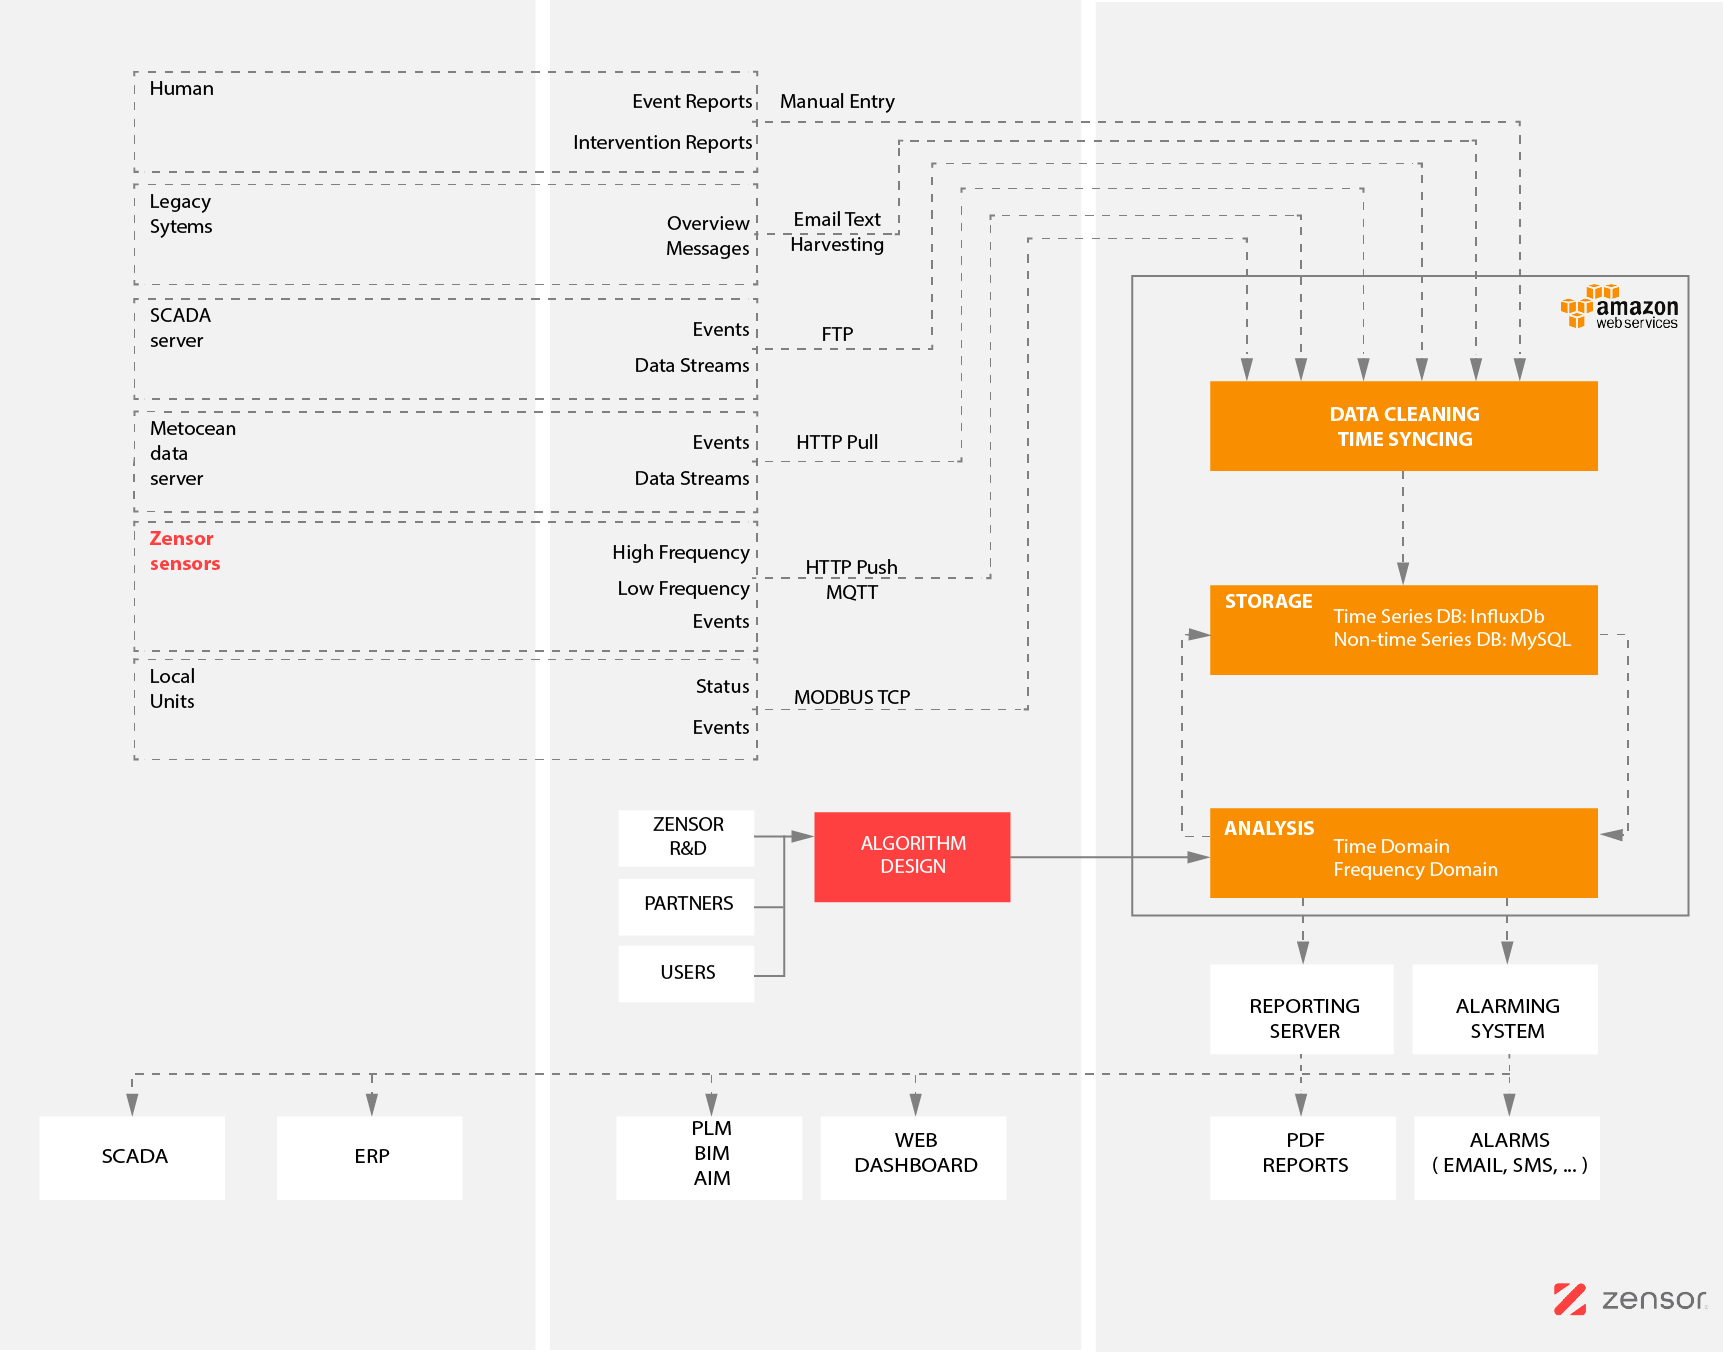
\includegraphics[width=\textwidth]{System_Architecture_Data Analytics.png}
    \caption{Zensor's system architecture for data analytics}
    \label{fig:zensor_sys_architecture}
\end{figure}
Making the assumption that the first two steps have gone well, we make a simplified scenario: the sensors of project \textit{22001\_XXX} have been properly installed and wired to the IPCs, programmed by the engineering team to collect data and aggregate it into files. 
We could say that the ``pump'' from the data lake\footnote{type of data repository that stores large and varied sets of raw data in its native format: \url{https://www.redhat.com/en/topics/data-storage/what-is-a-data-lake}} is up and running, but now the ``pipelines'' 
need to be built. As interesting a discussion as this is, this is likely to get off topic. To stay at a shallow level let's take a look at figure~\ref{fig:zensor_sys_architecture}; it shows us that:
\begin{itemize}
	\item The possible data sources, including our sensor data, are varied not to mention the formats or what protocols are used for managing transfer. 
	\item All ``roads'' lead to \textcolor{orange}{\ac{AWS}}, ensuring that each client will then have its own separate and independent cloud VM, with its own domain.
		This is where various things happen:\begin{enumerate}
		\item raw data gets cleaned, time synced and ingested in \ac{S3}\footnote{AWS an Object-Storage service. It is not a file system, instead, is a 'Key-Value' store} as backup system;
		\item most of the continuous analysis, also designed and implemented by zensor R\&D, is performed;
		\item multiple services are running, like database and web dashboard instances, see InfluxDB \ref{section:influxdb} and Grafana \ref{section:grafana} respectively.
	\end{enumerate} 
	\item \todo{DG: completare questa sezione}
\end{itemize}
We will give more space to some technical details later in chapter \ref{chapter:use_cases}. 

%\todo{DG:questa sezione è sicuramente da rivedere, magari da rimuovere?}
\subsubsection{Analysis: Structure of a Deployable Script}\label{subsection:script_structure}

\todo{DG:accennare a zensor library}
% https://www.notion.so/zensor/Zensor-library-90259840e02349a7adc5cb2a48abf994

\begin{figure}
	\[\begin{tikzcd}
		&& Datasource \\
		&& {} \\
		Load && Process && Write
		\arrow[from=3-1, to=3-3]
		\arrow[from=3-3, to=3-5]
		\arrow[from=1-3, to=3-1]
		\arrow[from=3-5, to=1-3]
	\end{tikzcd}\]
	\caption{Analysis script structure}
	\label{tik:analysis_script}
\end{figure}

Most scripts that run on the Zensor platform have a very common structure~\ref{tik:analysis_script}, so for a given time window, they:
\begin{enumerate}
	\item Load batch of data (either raw or from InfluxDB).
	\item Process it in some (clever!) way, e.g.\ computing a derived metric.
	\item Write the results out to InfluxDB, to be shown in a dashboard.
\end{enumerate}
What time window they operate on will depend on what the task is, but also on whether the script is being invoked automatically by cron, a job scheduler on Unix-like OS, or manually.
If a script is being invoked \textit{manually}, this is usually to run it over historical data (e.g.\ rerunning a script for the month of February 2022). We typically call this operation \textbf{backfilling}.
Typically, if the script is running in \textit{cron}, it's loading ``recent'' data (e.g.\ from the past hour or past day) ending at the time the script started.
Scripts on the Zensor platform need to support running in both modes, so there are a few guidelines to keep in mind when writing code.

